\chapter{Introduction to Computer Security}
\label{ch:intro_security}

\section{Introduction}
Computer security is often perceived by the general public through the lens of dramatic media representations, but at its core, it is fundamentally an engineering problem. The discipline is driven by a few basic but profound questions: What constitutes a secure system? How do we define computer security? And, most importantly, how do we engineer systems to be secure?

\section{The CIA Paradigm: Basic Security Requirements}
To meaningfully discuss and measure security, the industry relies on a foundational model known as the \textbf{CIA Paradigm} (or CIA Triad). This model defines three primary security requirements that must be upheld to consider a system secure:

\begin{itemize}
    \item \textbf{Confidentiality (C):} This principle ensures that information can be accessed only by authorized entities. Confidentiality is what protects sensitive data, such as personal user information or intellectual property, from being exposed to those who should not have it.
    \item \textbf{Integrity (I):} Integrity guarantees that information can be modified only by authorized entities, and only in ways that they are explicitly permitted to do so. This prevents unauthorized tampering, ensuring that data remains accurate and trustworthy.
    \item \textbf{Availability (A):} Availability ensures that information and system resources must be available to all authorized parties within specified, acceptable time constraints. A system that is perfectly confidential and perfectly integral but completely inaccessible is virtually useless.
\end{itemize}

A significant challenge in engineering secure systems is that these properties often conflict. For instance, maximizing Availability (e.g., making a system accessible from anywhere, at any time) inherently increases the attack surface, putting Confidentiality and Integrity at risk. Conversely, aggressively locking down a system to preserve Confidentiality can severely hinder Availability. Balancing these trade-offs is the essence of security engineering.

\section{Security as an Engineering Problem}
Treating security as an engineering discipline means moving away from absolute statements (like ``this system is unhackable'') and towards a structured understanding of vulnerabilities, threats, and risks. No system is truly invulnerable; thus, the goal is to systematically manage and mitigate these aspects. To do so, several key concepts must be defined: vulnerabilities, exploits, assets, threats, and risks.

\subsection{Vulnerabilities vs. Exploits}
It is crucial to distinguish between a vulnerability and an exploit. 

A \textbf{Vulnerability} is a weakness or flaw in a system that allows an attacker to violate one or more of the constraints of the CIA paradigm. It is the underlying condition that \textit{can} be abused.

An \textbf{Exploit}, on the other hand, is a \textit{specific way} to use one or more vulnerabilities to accomplish a specific objective that violates those constraints. It is the active application of a technique against the vulnerability.

\subsubsection{Physical Security Example: Lock Picking}
Consider a physical lock protecting a vault. A standard pin-tumbler lock may have a mechanical vulnerability due to imperfect manufacturing tolerances. When rotational pressure (torque) is applied to the lock's plug, not all pins bind simultaneously; one pin will bind first due to microscopic size discrepancies. 

The exploit for this vulnerability is the technique of \textit{lock picking}. An attacker uses a \textbf{tension wrench} to apply continuous torque to the plug. They then use a \textbf{pick} to lift the pins one by one. Because of the binding friction, once a pin is lifted to the \textbf{shear line} (the gap between the plug and the lock housing), it stays caught there. By repeating this process for all pins, the attacker aligns the shear line, and the lock opens.

\begin{figure}[htpb]
\centering
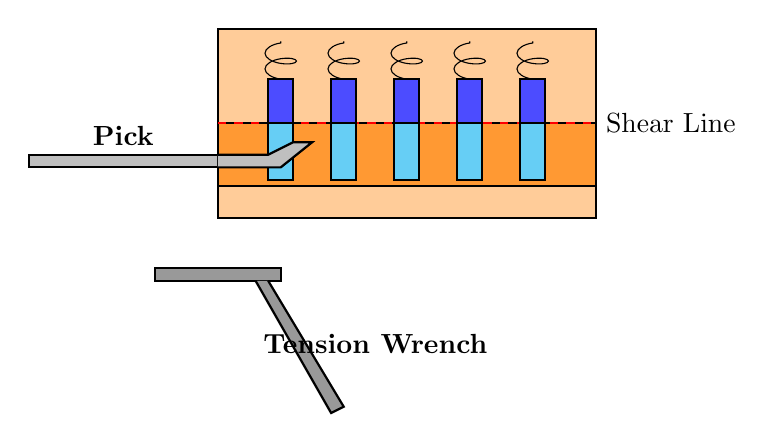
\begin{tikzpicture}[scale=0.8]
    % Outer housing
    \draw[fill=orange!40, thick] (0, 0) rectangle (6, 3);
    % Plug
    \draw[fill=orange!80, thick] (0, 0.5) rectangle (6, 1.5);
    
    % Shear line
    \draw[dashed, red, thick] (0, 1.5) -- (6, 1.5) node[right, text=black] {Shear Line};
    
    % Pins
    \foreach \x in {1, 2, 3, 4, 5} {
        % Bottom pin (key pin)
        \draw[fill=cyan!60, thick] (\x-0.2, 0.6) rectangle (\x+0.2, 1.5);
        % Top pin (driver pin)
        \draw[fill=blue!70, thick] (\x-0.2, 1.5) rectangle (\x+0.2, 2.2);
        % Spring
        \draw[decorate, decoration={coil, aspect=0.4, segment length=2mm, amplitude=2mm}] (\x, 2.2) -- (\x, 2.8);
    }
    
    % Pick tool
    \draw[fill=gray!50, thick] (-3, 0.8) rectangle (0, 1.0);
    \draw[fill=gray!50, thick] (0, 0.8) -- (1, 0.8) -- (1.5, 1.2) -- (1.2, 1.2) -- (0.8, 1.0) -- (0, 1.0);
    \node at (-1.5, 1.3) {\textbf{Pick}};
    
    % Tension Wrench
    \draw[fill=gray!80, thick] (-1, -1) rectangle (1, -0.8);
    \draw[fill=gray!80, thick] (0.8, -1) -- (2, -3) -- (1.8, -3.1) -- (0.6, -1);
    \node at (2.5, -2) {\textbf{Tension Wrench}};
    
\end{tikzpicture}
\caption{Simplified illustration of exploiting a physical lock. The tension wrench applies torque, creating binding friction. The pick lifts the pins to the shear line, exploiting mechanical tolerances (the vulnerability).}
\label{fig:lock_picking}
\end{figure}

To mitigate this, higher-quality locks introduce countermeasures like \textit{spool pins}, \textit{mushroom pins}, or \textit{serrated pins}. These do not eliminate the vulnerability entirely---the lock can still be picked---but they remove the feedback the attacker relies on, making the exploitation significantly more difficult and time-consuming.

\subsubsection{Software Security Example: Integer Truncation}
Software vulnerabilities often arise from seemingly innocuous programming mistakes. Consider the following simplified C code designed to authenticate a user based on an input number:

\begin{verbatim}
int i;
unsigned short s;

i = atoi(argv[1]); // parse command line parameter as int

if (i == 0) { // check
    printf("Invalid number: value must be > 0\n");
    return -1;
}

s = i; // implicit truncation

if (s == 0) { // security check
    printf("Access GRANTED!\n");
}
\end{verbatim}

\textbf{The Vulnerability:} The code validates the integer \texttt{i} to ensure it is not zero. In standard C, an \texttt{int} is typically 32 bits, while an \texttt{unsigned short} is only 16 bits. When \texttt{i} is assigned to \texttt{s}, the 32-bit integer is implicitly truncated to its lower 16 bits. The vulnerability is the combination of this unsafe type conversion and the subsequent security check relying on the truncated value.

\textbf{The Exploit:} An attacker can input a number that is not zero in 32 bits but becomes zero when truncated to 16 bits. Since $2^{16} = 65536$, running the program with the argument \texttt{65536} bypasses the first check (since $65536 \neq 0$). During the assignment \texttt{s = i}, the value \texttt{65536} (which in binary is a \texttt{1} followed by sixteen \texttt{0}s) is truncated. The lower 16 bits are all zero, so \texttt{s} becomes \texttt{0}. The final check \texttt{if (s == 0)} evaluates to true, and access is granted. Here, the number \texttt{65536} is the specific exploit.

\subsection{Assets, Threats, and Attacks}
To understand risk, we must map out what we are trying to protect and who we are protecting it from.

An \textbf{Asset} identifies what is valuable to an organization. In IT contexts, this includes:
\begin{itemize}
    \item \textbf{Hardware:} Laptops, servers, networking equipment.
    \item \textbf{Software:} Operating systems, custom applications, databases.
    \item \textbf{Data:} Customer records, intellectual property, financial ledgers.
    \item \textbf{Reputation:} The organization's standing, particularly regarding social media and public trust.
\end{itemize}

A \textbf{Threat} is a potential violation of the CIA paradigm---a circumstance or event capable of causing harm. Examples include Denial of Service (compromising Availability), Identity Theft (compromising Confidentiality/Integrity), or Data Leaks.

An \textbf{Attack} is the \textit{intentional} use of one or more exploits with the objective of compromising a system's CIA. For example, attaching a malicious PDF to an email or physically picking a lock to enter a server room.

A \textbf{Threat Agent} is the entity---whoever or whatever---that may cause an attack to occur, such as a malicious script, a rogue employee, or a physical thief.

\subsection{Demystifying Terminology: Hackers vs. Attackers}
The mass media has generated considerable confusion around security terminology. It is important to distinguish between these concepts.

An \textbf{Attacker} is anyone or anything that performs an attack.

A \textbf{Hacker}, historically and within the technical community, is someone with an \textit{advanced understanding} of computers and computer networks, driven by a deep willingness to learn ``everything'' about how systems work under the hood. 

An attacker is not necessarily a hacker (e.g., someone running a pre-packaged script without understanding it), and a hacker is not necessarily an attacker. When hackers use their skills maliciously, they are referred to as \textbf{Black Hats}. Conversely, \textbf{Security Professionals} or \textbf{White Hats} are ethical hackers. They use the same advanced skillset to:
\begin{itemize}
    \item Identify vulnerabilities.
    \item Develop exploits (to prove vulnerabilities exist).
    \item Develop attack-detection methods.
    \item Develop countermeasures.
    \item Engineer robust security solutions.
\end{itemize}

\section{Security as Risk Management}
Because no system is invulnerable, security cannot be treated as an absolute state. Instead, it is an exercise in \textbf{Risk Management}. 

\textbf{Risk} is defined as the statistical and economical evaluation of the exposure to damage resulting from the presence of vulnerabilities and threats. It can be conceptually modeled as:

\[ \text{Risk} = \text{Asset} \times \text{Vulnerabilities} \times \text{Threats} \]

In this equation:
\begin{itemize}
    \item \textbf{Threats} are generally an \textit{independent variable}. An organization usually cannot control whether malicious actors decide to target them.
    \item \textbf{Assets} and \textbf{Vulnerabilities} are \textit{controllable variables}. An organization decides what assets to put online and how rigorously to patch and secure them.
\end{itemize}

A highly vulnerable system facing zero threats might have a low overall risk, while a reasonably secure system facing persistent, advanced threats might have a high risk.

\subsection{The Balance of Security vs. Cost}
Engineering security means reducing vulnerabilities and planning for damage containment, but this must always be balanced against \textbf{cost}. Throwing more money at a problem does not inherently yield more security. For example, a highly expensive but improperly configured firewall provides a false sense of security and is arguably worse than having no firewall.

Costs are categorized into:
\begin{itemize}
    \item \textbf{Direct Costs:} Management overhead, operational expenses, and equipment purchases.
    \item \textbf{Indirect Costs (often more relevant):} Decreased usability, slower system performance, reduced user privacy due to invasive monitoring, and reduced overall productivity.
\end{itemize}

If security controls are too expensive in terms of usability (e.g., overly complex password policies requiring frequent changes), users will inevitably circumvent them (e.g., by writing passwords on sticky notes), effectively nullifying the security investment.

\section{Trust and Assumptions}
At the foundation of any secure system, boundaries must be set. Within these boundaries, certain elements must simply be \textit{assumed} secure. These form the \textbf{trusted elements} of the system. 

When evaluating a system, we must ask: Can we trust the security officer? The newly installed software? Our own code? The compiler? The BIOS? The hardware itself?

This creates a ``chicken and egg'' chain-of-trust problem. This paradox was famously explored by Ken Thompson in his 1984 Turing Award lecture, \textit{"Reflections on Trusting Trust"}. Thompson demonstrated how a compiler could be modified to insert a backdoor into programs it compiled (like the \texttt{login} command), and further, how the compiler could recognize when it was compiling \textit{itself} and insert the backdoor-generation code into the newly compiled compiler. The malicious source code could then be removed from the compiler's source tree, leaving no trace, yet the binary compiler would perpetually reproduce the vulnerability. This highlights that unless you bootstrap an entire system yourself from basic principles (as initiatives like \texttt{bootstrappable.org} attempt to do), you are ultimately placing blind trust in some foundational level of the technology stack.

\section{Conclusions}
Computer security is a complex engineering discipline focused on balancing conflicting requirements (Confidentiality, Integrity, Availability) against practical limitations and costs. It requires a nuanced understanding of risk management, where vulnerabilities must be weighed against actual threats and the value of the underlying assets. Recognizing the distinction between vulnerabilities and exploits, and between malicious attackers and skilled hackers, is crucial for developing effective countermeasures. Ultimately, because absolute security is unattainable and trust must invariably be placed somewhere in the supply chain, security remains an ongoing process of risk mitigation rather than a solvable destination.
